\documentclass[twoside=false,DIV=14]{scrartcl}

\usepackage{arev} % order matters, putting this above allows FiraSans to override it for body text
\usepackage[sfdefault]{FiraSans}
\usepackage{inconsolata}
%\usepackage[fira]{fontsetup}
\usepackage{scrlayer-scrpage}
\renewcommand{\titlepagestyle}{scrheadings}
\usepackage{graphicx}
\usepackage{blindtext}
\usepackage{wrapfig}
\usepackage{tabularx}
\usepackage{hyperref}
\usepackage{listings}
\usepackage{tikz}
\usepackage{amsmath}
\usepackage[many]{tcolorbox}

\usepackage{xcolor,sectsty}
\definecolor{blackish}{RGB}{56,58,54}
\definecolor{redish}{RGB}{109,41,49}
\definecolor{red}{RGB}{152,41,50}
\definecolor{orangeish}{RGB}{188,71,0}
\definecolor{blueish}{RGB}{25,33,139}
\subsubsectionfont{\color{blackish}}
\subsectionfont{\color{blackish}}
\sectionfont{\color{blackish}}

\lohead{\color{red} COMP3000 Programming Languages}
\rohead{
\includegraphics[width=0.5cm]{../logo.jpg}}

\setkomafont{author}{\sffamily \small}
\setkomafont{date}{\sffamily \small}

\DeclareOldFontCommand{\bf}{\normalfont\bfseries}{\mathbf}
\DeclareOldFontCommand{\tt}{\normalfont\ttfamily}{\texttt}

\lstset{basicstyle=\ttfamily}


\date{}
\newtcolorbox{aside}[1][]{
  title=Aside,
  width=0.3\textwidth,
  fonttitle=\bfseries,
  breakable,
  fonttitle=\bfseries\color{black},
  colframe=blueish!80,
  colback=blueish!2
  #1}

\newtcolorbox{note}[1][]{
  title=Note,
  width=\textwidth,
  fonttitle=\bfseries,
  breakable,
  fonttitle=\bfseries\color{black},
  colframe=orangeish!80,
  colback=orangeish!2
  #1}

\newtcolorbox{hint}[1][]{
    title=Hint,
    width=\textwidth,
    fonttitle=\bfseries,
    breakable,
    fonttitle=\bfseries\color{white},
    colframe=blueish!80,
    colback=blueish!2
    #1}

\newtcolorbox{todo}[1][]{
  title=!! TODO !!,
  width=\textwidth,
  fonttitle=\bfseries,
  breakable,
  fonttitle=\bfseries\color{white},
  colframe=red!80,
  colback=red!2
  #1}
  
\providecommand{\tightlist}{%
  \setlength{\itemsep}{0pt}\setlength{\parskip}{0pt}}


\title{\color{redish} \vspace{-2em}Week 2 Workshop: Review, Recursion, and Iteration}

\begin{document}
{\color{blackish}\maketitle}\vspace{-2em}%\input{proposal.inc}
\begin{itemize}
    \item[$\cdot$] {\bf Resources:}  Week 1 Diagnostic Quiz and Code Bundle.
    \item[$\cdot$] {\bf To submit this week's work:} Submit your solution to Exercise 3 to your teacher in class.  You should hand in a single piece of paper with your solution on it.  Be sure you include your name, student number, and the week number in the top-right of your submission.
\end{itemize}
Questions that ask about linked lists are asking about the \emph{concept} of linked lists we spoke about in the lecture and which we \emph{implemented} in our \lstinline|LinkedList| class.  There are infinitely many different linked list implementations, please use ours.


\part*{Exercises}
    

\section{Java Review: Definitions}

As precisely as you can, define the following terms (which you learned in COMP1010):
    \begin{enumerate}
    \item method
    \item class
    \item reference
    \item value
    \end{enumerate}

\section{Java Review: Java Program}
Write a Java program which reads data from the user on the console and stores each response they give.  When the user gives the special response "over and out", the program will replay their responses.
    
    An example interaction would be

    \begin{lstlisting}
    > ? hi
    > ? my
    > ? knee is
    > ? sore
    > ? over and out
    hi my knee is sore
    \end{lstlisting}

    You may assume there will be no more than 10 lines input before "over and out" is input.

\section{Recursive Data: Concepts - \bf Submission}
    Draw diagrams of the three linked lists that result from the following code being executed.

    \begin{lstlisting}
        LinkedList small = new LinkedList('m');
        
        LinkedList matt = 
               new LinkedList('m', 
                 new LinkedList('a', 
                   new LinkedList('t', 
                     new LinkedList('t'))));
        
        LinkedList notMatt = new LinkedList('s');
        notMatt.add('o');
        notMatt.add('m');
        notMatt.add('e');
        notMatt.add('o');
        notMatt.add('n');
        notMatt.add('e');
        notMatt.add('e');
        notMatt.add('l');
        notMatt.add('s');
        notMatt.add('e');
      \end{lstlisting}  


\section{Recursive Data: More}    
We've seen that linked lists are a type of recursive data.  In this task we will try to come up with some other type of recursive data and think about how it might be structured.  Recall
    \begin{quote}
    Recursion refers to the situation where the smaller part shares key characteristics of the whole.
    \end{quote}
    We chose to use linked lists of characters because \emph{Strings} are another type of recursive data.  A string missing one of its characters is also a string!  Thinking along those lines, think of another kind of data that could be treated recursively.

    Note:  This will require either imagination or some research since you haven't seen that many other data types so far. 
    
\section{Recursion: Write a recursive function}
Write a \emph{concatenation} function for the \lstinline|LinkedList| class.  The method should concatenate the given list to \lstinline|this| list, updating \lstinline|this| in-place.  The method signature should be:
    \begin{lstlisting}
    void concat(LinkedList other);
    \end{lstlisting}
    and it should pass \emph{at least} the following tests (assuming the definitions of \lstinline|small|, \lstinline|matt|, and \lstinline|notMatt| from above)
    \begin{lstlisting}
      matt.concat(notMatt);
      matt.concat(small);
      
      assertTrue(matt.toString().equals("mattsomeoneelsem"));
    \end{lstlisting}

\section{Recursion Iteration Iso: Iterative Version}
Write an iterative version of the \lstinline|concat| function you wrote above.
    
    \newpage\setcounter{section}{0}
\part*{Solutions}
    \subsection*{Notes on solutions}

    \begin{description}
    \item[Why does Matt give code listings in a PDF instead of the code files?]  Nobody ever learned anything new by downloading a file.  The act of typing in the code yourself is a key part of learning.  Of course, you certainly must take care to only spend time on valuable learning experiences as you have busy lives, but typing out relatively small Java examples \emph{is} a valuable way to learn.
    \end{description}

    
\section{Java Review: Definitions}
    My answers are:
      \begin{description}
      \item [method] A function defined on an object.  Has an implicit \lstinline|this| variable available.
      \item [class] The templates from which Objects are built.  Also bring new types into existence.
      \item [reference] A pointer to a slot in memory.
      \item [value] In Java these are any things that fit in one slot of memory, precisely those are integers, booleans, characters, and references to objects.
      \end{description}
  
\section{Java Review: Write some code}
    I've chosen to use \lstinline|java.util.Scanner| to get user input but there \emph{are} other methods.  This is a good example to get you back on your coding toes because:
    \begin{itemize}
    \item You might not have seen \lstinline|java.util.Scanner| before, so you can practice learning new methods.
    \item You need to declare things in just the right places.
    \item If you are careful with your loop condition you can make your code neater
    \item If you make that work well with your \lstinline{used} variable it gets even neater.
    \item You need to do some very simple array work, prepping us for the recursive work.
    \end{itemize}
    Many solutions are possible, here is mine.
    \begin{lstlisting}
  package week1;

  import java.util.Scanner;

  public class Workshop2Parrot {
    public static void main(String[] args){
        String[] inputs = new String[10];
        int used = 0;
        Scanner s = new Scanner(System.in);
        String response = "";
        while(used < 10 && !response.equals("over and out")){
            System.out.print("? ");
            response =s.nextLine();
            inputs[used] = response;
            used++;
        }
        for (int i = 0; i < used -1; i++){
          System.out.print(inputs[i]);
          System.out.print(" ");
        }
        System.out.println();
    }   
  }

    \end{lstlisting}
\section{Recursive Data: Concepts - Submission}

Note, I use the symbol $\phi$ for \lstinline|null|.\\
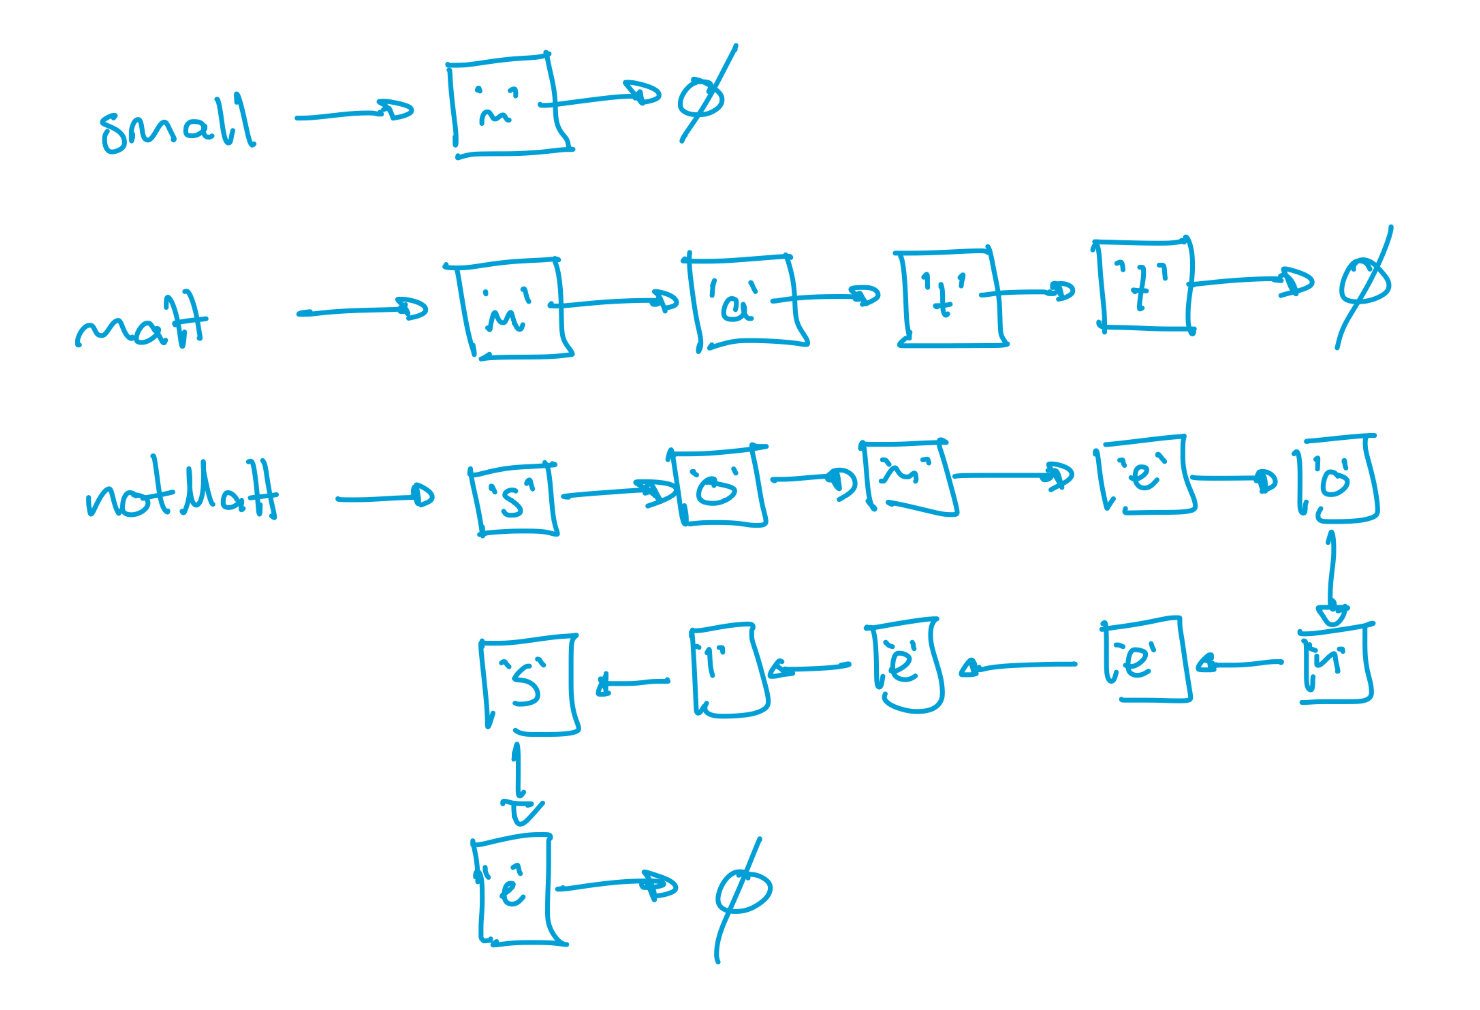
\includegraphics[width=\textwidth]{./week2_1.png}

\section{Recursive Data: More}
Note: this task gives you the opportunity to practice getting things off the web in a constructive manner.  I am willing to bet many students types "recursive data type" into google or ChatGPT in attempting to answer this question.  That is fine, but the next step is critical.  The next step is to assimilate the answer and construct your own understanding from it.
    
    I ended up going with \emph{spreadsheets}.  If you remove a row from a spreadsheet, the result is still a spreadsheet right?

    Other options students might think of are:
    \begin{description}
    \item[arrays] It works, but you are really just doing linked lists with that example
    \item[concepts from databases] in those courses they will have seen tables, and you can always take one row from a table to get another table.  Thus they might say "classroom - if you take a student from a classroom, you still have a classroom", etc.
    \end{description}
    I tried out Microsoft Copilot.  Copilot \emph{insists} on talking about trees when I ask.  These \emph{are} recursive data but the students haven't learned them yet!  I guess they \emph{could} come to understand them in answering this question, but it is worth prompting to see if they really get it or if they are parroting a partly understood answer from the web.  The habit of partly understading whatever the internet said is kryptonite to learning and a habit to be broken as soon as possible!  I really pushed the LLMs and never got an answer that was readily understandable by a second year student.  When I pushed copilot on s-expressions (one of the suggestions it made) it gave incorrect information and doubled down on it.   Thus, I can say (at the moment) Copilot does not understand the subtle, but important, difference between iterative data and recursive data and thus is a bad study-partner in this particular case. We will continue to keep an eye on the LLMs during semester to see if they are helpful or harmful for our learning.

\section{Recursion : Write a recursive function}
I will give the recursive solution first 
\begin{lstlisting}
void concat(LinkedList other){
    if (next == null){
        next = other;
    } else {
        next.concat(other);
    }
}
\end{lstlisting}
For both this and the next solution, a solid understanding of \emph{references} in Java is needed.  If you are struggling with this question even though you are comfortable with linked lists and recursion, that is likely to be your problem.

\section{Recursion Iteration Iso}
Since we did recursive in the last answer, let's do iterative here
\begin{lstlisting}
void concat_iterative(LinkedList other){
    LinkedList curr = this;
    while(curr.next != null){
        curr = curr.next;
    }
    curr.next = other;
}
\end{lstlisting}
  
  \newpage\setcounter{section}{0}

  \part*{Self Study Exercises}

  \section{Recursion: Splitting}
  Write a recursive function \lstinline|LinkedList splitAt(char c)| that splits a linked list at a given value.  After splitting, the original linked list is shorted and a new linked list is returned holding the remaining part of that linked list.  If the value is not in the linked list, or it is the last value of the linked list, the list is not changed and \lstinline|null| is returned.

  \section{Recursion Iteration Iso: Splitting iteratively}
  Write an iterative version of the \lstinline|splitAt| function you wrote above.

  \section{Recursion: Concepts}
  What makes the first solution recursive while the second one is iterative?  Be clear and concise in  your answer.

  \section{Recursion: Zipping}
  Write a recusive function on the \lstinline|zipWith| class which "zips" the linked list with some other linked list.  "Zipping" lists means taking one element from the first, then one from the second, then one from the first, etc.  The function does not change the existing lists, it returns a brand new list.  Here are some example input/output pairs:
  \begin{itemize}
  \item \lstinline|notMatt.zipWith(notMatt)| gives \lstinline|ssoommeeoonneeeellsse|
  \item \lstinline|matt.zipWith(notMatt)| gives \lstinline|msaotmeoneelse|
  \end{itemize} 

  To further clarify, if you start with these two lists\\
  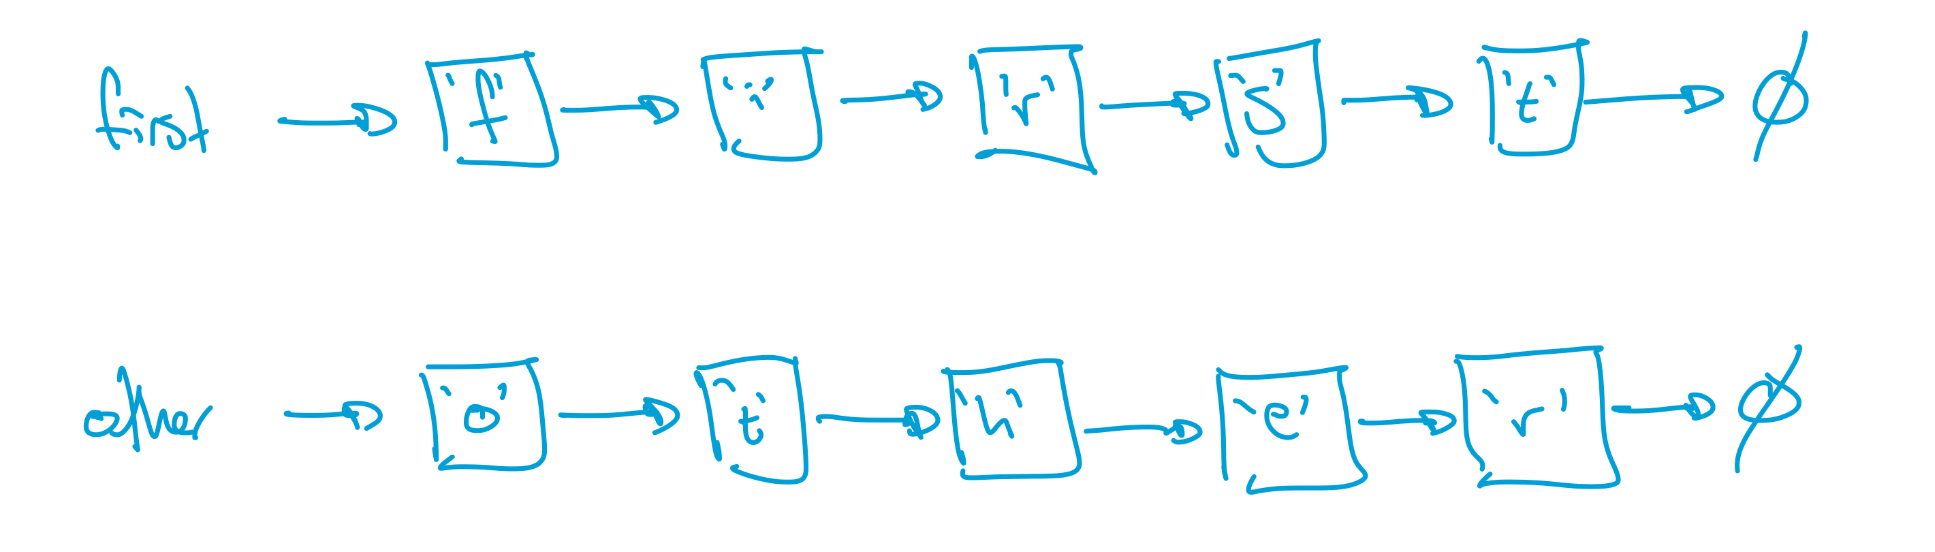
\includegraphics[width=\textwidth]{./week2_2.png}\\
  the end result will be the following list\\
  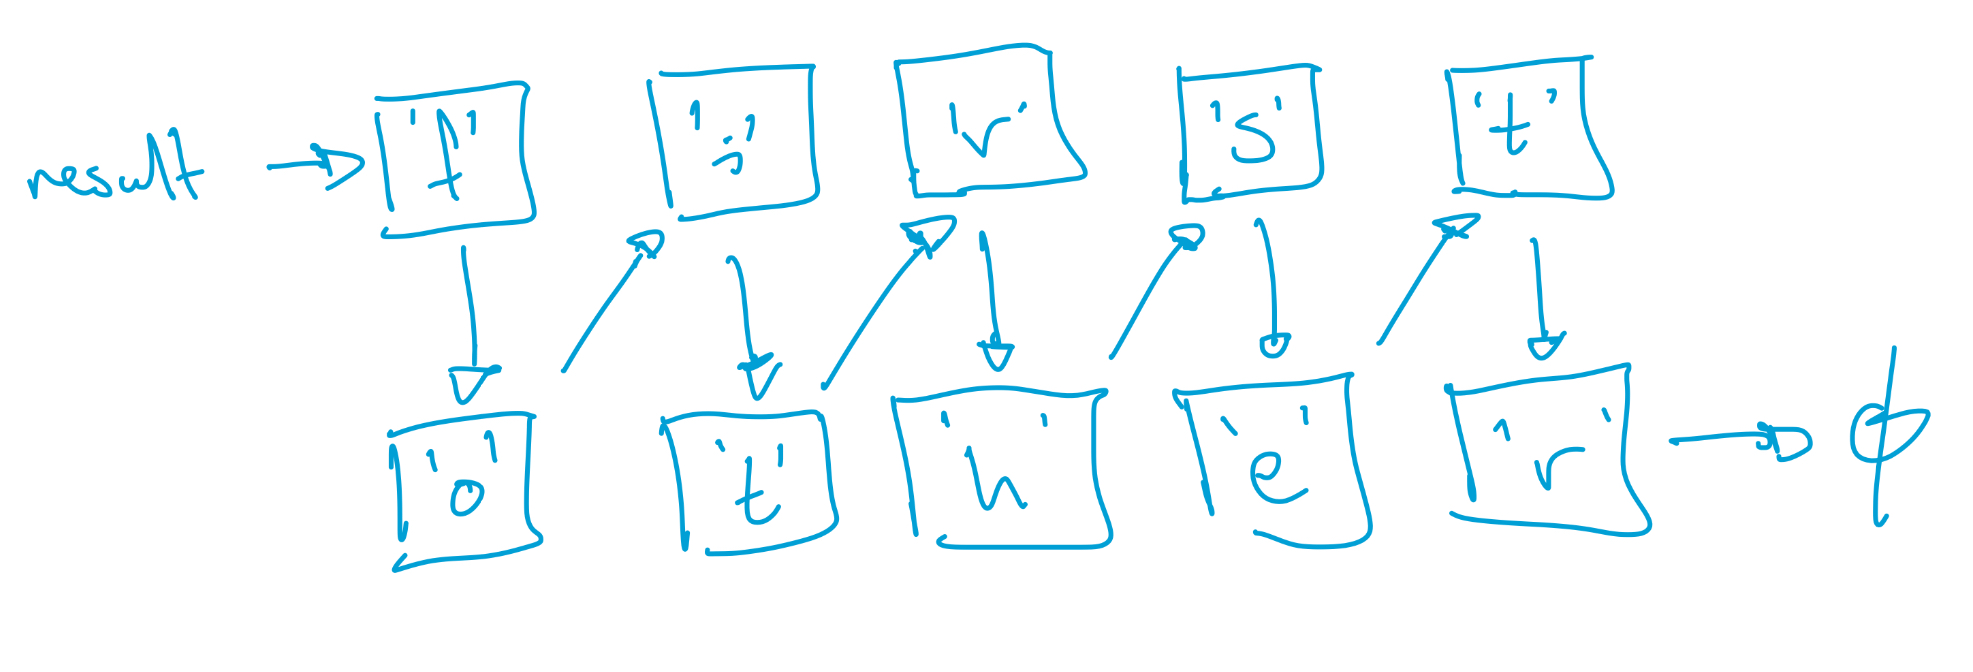
\includegraphics[width=\textwidth]{./week2_3.png}

  \section{Recursion Iteration Iso: Zipping (Hard)}
  Write an iterative version of the \lstinline|zipWith| function.

  \section{Java Proficiency: Testing}
  Write a few basic test functions to try out your \lstinline|zipWith| function.  No need to be comprehensive, but make sure your tests are convincing evidence that the code is right.
  
  \newpage\setcounter{section}{0}
  \part*{Self Study Solutions}
  \section{Recursion: Splitting}
  \begin{lstlisting}
    LinkedList splitAt(char c){
      if (next == null){
          return null;
      } else {
          if (value == c){
              LinkedList ret = next;
              next = null;
              return ret;
          } else {
              return next.splitAt(c);
          }
      }
    }
  \end{lstlisting}
  \section{Recursion Iteration Iso: Splitting iteratively}
  \begin{lstlisting}[language=java]
    LinkedList splitAt_iterative(char c){
        LinkedList curr = this;
        while(curr != null){
            if (curr.value == c){
                LinkedList ret = curr.next;
                curr.next = null;
                return ret;
            }
            curr = curr.next;
        }
        return null;
   }
  \end{lstlisting}

  \section{Recursion: Concepts}
  Recall that recursion is the concept that the part has the same characteristics as the whole.  In the recursive solution we rely on this fact when we call \lstinline|next.splitAt()|.  I.e. the fact that we call the very same function on a part of the whole indicates it is recursive.  

  In the iterative solution we never do a splitting on the part, we inspect the subparts one by one until we find the place to split.  Whenever we process "one by one", we are acting iteratively.

  \section{Recursion: Zipping}
  The recursive solution can take some time to get your head around, but it is quite neat once you get it.
  \begin{lstlisting}
  LinkedList zipWith(LinkedList other){
        if (next == null){
            return new LinkedList(this.value, other);
        } else if (other == null){
            return this;
        } else {
            return new LinkedList(this.value, other.zipWith(this.next));
        }
   }
  \end{lstlisting}

  \section{Recursion Iteration Iso: Zipping (Hard)}
  I'll be honest, I could not find a good iterative solution to this one.  The recursive solution was so neat and my iterative solution is a mess!  This is not unsurprising since recursion suits some problems and iteration suits others.  So far we've only seen problems that work well both ways, but that's just because we are easing into it.  If you've found a neat solution, pass it on to us for prize points.
  \begin{lstlisting}
  LinkedList zipWith_iterative(LinkedList other){
        LinkedList curr = new LinkedList(this.value);
        LinkedList on = other;
        LinkedList me = this.next;
        while(me != null && other != null){
            curr.add(on.value);
            if (on == me){
                me = me.next;
                on =  other;
            } else {
                other = other.next;
                on = me;
            }
        }
        if (me == null){
            curr.concat(other);
        }
        if (other == null){
            curr.concat(me);
        }
        return curr;
   }

  \end{lstlisting}
  \section{Java Proficiency: Testing}
  I've covered three different possible situations:
  \begin{enumerate}
  \item both lists the exact same length
  \item lists of different lengths
  \item one of the lists is empty
  \end{enumerate}
  And I have tested each combination in each direction and with each version of \lstinline|zipWith|.

  Just for fun, I mixed up the different ways of constructing lists.
  \begin{lstlisting}
  @Test
  public void zipExample(){
    LinkedList first = new LinkedList('f', 
                       new LinkedList('i', 
                       new LinkedList('r', 
                       new LinkedList('s', 
                       new LinkedList('t')))));
    LinkedList other = new LinkedList('o', 
                       new LinkedList('t', 
                       new LinkedList('h', 
                       new LinkedList('e', 
                      new LinkedList('r')))));
    assertEquals(first.zipWith(other).toString(), "foitrhsetr");
    assertEquals(other.zipWith(first).toString(), "oftihresrt");
    assertEquals(first.zipWith_iterative(other).toString(), "foitrhsetr");
    assertEquals(other.zipWith_iterative(first).toString(), "oftihresrt");
  }

  @Test
  public void differentLengths(){
    LinkedList small = new LinkedList('s', new LinkedList('m'));
    LinkedList longer = new LinkedList('l');
    longer.add('l');
    longer.add('o');
    longer.add('o');
    longer.add('o');
    longer.add('n');
    longer.add('g');
    assertEquals(small.zipWith(longer).toString(), "slmlooong");
    assertEquals(longer.zipWith(small).toString(), "lslmooong");
    assertEquals(small.zipWith_iterative(longer).toString(), "slmlooong");
    assertEquals(longer.zipWith_iterative(small).toString(), "lslmooong");
  }

  @Test
  public void empty(){
    LinkedList empty = null;
    LinkedList single = new LinkedList('s');
    assertEquals(single.zipWith(empty).toString(), "s");
    assertEquals(single.zipWith_iterative(empty).toString(), "s");
  }
  \end{lstlisting}
  \end{document}